\RequirePackage[l2tabu,orthodox]{nag}
\documentclass[10pt,twocolumn,a4paper,os=win]{article}

\usepackage[utf8]{inputenc}
\usepackage[T1]{fontenc}
\usepackage[english]{babel}
\usepackage{lmodern}
\usepackage{microtype}
\usepackage{parskip}
\usepackage{amsmath}
\usepackage{amssymb}
\usepackage{mathtools}
\usepackage{csquotes}
\usepackage{graphicx}
\usepackage{tikz}

\usepackage[margin=2cm]{geometry}

\usepackage[
	backend=biber
]{biblatex}
\addbibresource{gui.bib}

\usepackage{menukeys}

\usepackage[hidelinks]{hyperref}

%\raggedbottom

\author{Markus Himmel}
\title{Windows GUI}

\newcommand{\bs}[1]{\textbf{\sffamily #1}}
\newcommand{\winver}[1]{$^{\text{\hyperref[tbl:abbrev]{\bs{#1}}}}$}

\begin{document}
	\maketitle

	\begin{abstract}
		The Graphical User Interface is one of the most important components
		of a consumer-oriented operating system such as Microsoft Windows. This
		report examines the components of the Windows operating system that
		contribute to the graphical user interface, both from an application
		programmer's and a system architect's point of view. % TODO: Expand
	\end{abstract}

	\section{Introduction}
		% TODO: Annoying stuff

		Rigorously defining requirements for an efficient graphical user
		interface is outside the scope of this report. Instead, we will focus
		on one particular aspect: Responsiveness. Users perceive the response
		of a computer as \enquote{instantaneous} if the response time is less
		than 100 milliseconds \cite{miller1968response}. Ensuring that as
		little of that time as possible is used for drawing the application on
		the screen is key to the usability of a graphical user interface.

		\subsection{How to read this document}
			The Windows operating system has seen many revisions over its
			decades-long lifespan, and many of the features described in this
			report differ significantly from version to version. At the same
			time, documentation of the architecture of the Windows GUI is
			scarce at best.  For this reason, it is not possible to present an
			entirely consistent exposition of the Windows GUI architecture of
			some fixed Windows version.  Instead, different sections of this
			report may be based on different versions of Windows. In order to
			aid the reader in keeping track of which version of Windows is
			being examined at any given point in time, sections and sometimes
			single paragraphs and sentences will be marked with the Windows
			versions they describe. Here is an example:

			GDI is not hardware-accelerated.\winver{V}

			Table~\ref{tbl:abbrev} lists all abbreviations used in this document
			and the Windows versions they refer to.

			\begin{table}[h]
				\centering
				\begin{tabular}{r|l}
					Abbreviation & Windows Version \\
					\hline
					\bs{3} & Windows NT 3.51 \\
					\bs{4} & Windows NT 4.0 \\
					\bs{XP} & Windows XP \\
					\bs{V} & Windows Vista (\enquote{Longhorn}) \\
					\bs{7} & Windows 7 \\
					\\
					\bs{WRK} & Windows research kernel \\
					\bs{R} & ReactOS source code
				\end{tabular}
				\caption{Abbreviations for Windows versions used in
					this document}
				\label{tbl:abbrev}
			\end{table}

			In some cases, no documentation of a particular implementation detail
			may exist for any Windows version. In this situation, the author of
			this report used the source code of the ReactOS project in order to
			at least present \emph{a} implementation, without intending to imply
			that this implementation is similar to that of any real Windows
			version.

	\section{Win32 GUI applications}
		\subsection{Window objects}

		\subsection{Window messages and procedures}

	\section{NT Kernel support for GUI applications}\label{sec:win32k}
		\begin{figure*}
			\centering
			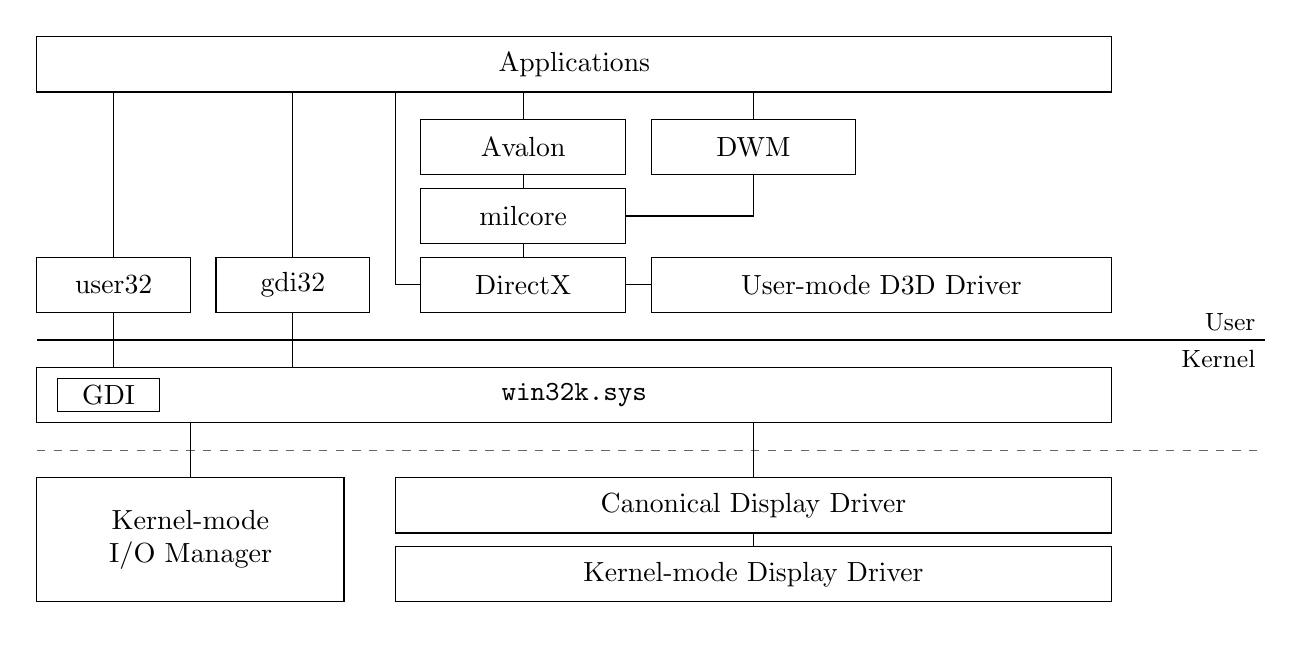
\begin{tikzpicture}[yscale=0.7, xscale=1.3]
				\node at (0, 0) {};
				\node at (12, 10.5) {};
				\draw[thick] (0, 5) -- (12, 5);
				\node[anchor=south east] at (12, 5) { \small User };
				\node[anchor=north east] at (12, 5) { \small Kernel };
				\draw (0, 9.5) rectangle node (apps) { Applications } ++(10.5, 1);
				\draw (0, 5.5) rectangle node { user32 } ++(1.5, 1);
				\draw (0.75, 6.5) -- ++(0, 3);
				\draw (0, 3.5) rectangle node { \texttt{win32k.sys} } ++(10.5, 1);
				\draw (0.75, 4.5) -- ++(0, 1);
				\draw (0, 0.25) rectangle node[align=center,text width=2.5cm] { Kernel-mode I/O Manager } ++(3, 2.25);
				\draw[dashed,color=black!60] (0, 3) -- (12, 3);
				\draw (1.5, 2.5) -- ++(0, 1);
				\draw (1.75, 5.5) rectangle node (gdi32) { gdi32 } ++(1.5, 1);
				\draw (2.5, 6.5) -- ++(0, 3);
				\draw (2.5, 4.5) -- ++(0, 1);
				\draw (0.2, 3.7) rectangle node { GDI } ++(1, 0.6);
				\draw (3.5, 0.25) rectangle node { Kernel-mode Display Driver } ++(7, 1);
				\draw (3.5, 1.5) rectangle node { Canonical Display Driver } ++(7, 1);
				\draw (7, 2.5) -- ++(0, 1);
				\draw (7, 1.25) -- ++(0, 0.25);
				\draw (3.75, 5.5) rectangle node { DirectX } ++(2, 1);
				\draw (3.75, 6.75) rectangle node { milcore } ++(2, 1);
				\draw (6, 5.5) rectangle node { User-mode D3D Driver } ++(4.5, 1);
				\draw (3.75, 8) rectangle node { Avalon } ++(2, 1);
				\draw (3.75, 6) -| ++(-0.25, 3.5);
				\draw (4.75, 9) -- ++(0, 0.5);
				\draw (4.75, 7.75) -- ++(0, 0.25);
				\draw (4.75, 6.5) -- ++(0, 0.25);
				\draw (5.75, 6) -- ++(0.25, 0);
				\draw (6, 8) rectangle node { DWM } ++(2, 1);
				\draw (7, 9) -- ++(0, 0.5);
				\draw (5.75, 7.25) -| ++(1.25, 0.75);
			\end{tikzpicture}
			\caption{An overview of the Windows GUI architecture, showing both user-mode
				and kernel-mode components involved in rendering the Windows GUI}
			\label{fig:arch}
		\end{figure*}

		The functions available to the user for creating GUI applications are
		exported by \texttt{user32.dll}, which is a user-space library.
		However, the actual functionality is provided by a kernel module called
		\texttt{win32k}. Refer to figure~\ref{fig:arch} for an overview over the
		components involved in the Windows Graphical User Interface. \cite{probertwin32k}

		\subsection{Moving \texttt{win32k} to the kernel\winver{4}}
			It is possible to provide functionality described in section~\ref{sec:win32k}
			using a user space module. Even further, proper microkernel design principles
			mandate that \texttt{win32k} \emph{must} be placed in user space, merely
			because it can. In fact, Windows versions prior to Windows NT 4.0
			did implement \texttt{win32k} functionality in user space. However,
			in Windows NT 4.0 \texttt{win32k} was moved to kernel space for
			performance reasons. Windows NT 3.51 contains large number of optimizations
			to be able to support a user-space \texttt{win32k}, many of them related
			to efficient execution of GDI operations (cf. section~\ref{sec:gdi}).
			For example, GDI operations requested by the applications are not
			actually drawn immediately by calling into the kernel and communicating
			with the graphics hardware. Instead, GDI operations are placed in a
			queue. Once the queue is full or is flushed manually by the application,
			the switch into kernel mode is made and all queued operations are executed
			in sequence. Symetrically, \texttt{win32k} data which is available to the application
			is cached in user space.
			Many (though not all) of these optimizations become unnecessary when
			\texttt{win32k} is moved into kernel space, achieving a simpler implementation
			with improved performance.
			\cite{gdikernel}

			The architectural justification for this change is that the subsystem
			retains its microkernel-like interface while providing significantly
			improved performance. This style of kernel architecture is referred
			to as \emph{modified microkernel}. \cite{gdikernel}

			Moving \texttt{win32k} from user mode to kernel mode without fundamentally
			adapting its architecture---which would be very challending due to
			compatibility---has created an entire class of security problems.
			In several situations arising in the context of \texttt{win32k},
			calling back from the kernel into user mode code (rather than just
			returning) is necessary. In order to facilitate this, \texttt{win32k}
			provides a mechanism called \textit{user-mode callbacks}. This
			functionality has shown to be very prone to creating security problems,
			such as information leakage or transitioning back into user mode after
			a different code execution vulnerability has already been exploited.
			\cite{mandy2011kernel}

	\section{Win32 drawing APIs}
		\subsection{Graphics Device Interface} \label{sec:gdi}

		\subsection{DirectX}

		\subsection{Avalon}\label{sec:milcore}

		\subsection{OpenGL}

		% TODO: Vulkan, Metal, ...

	\section{Window Management}
		\subsection{Window managers and compositing}
			The window manager is the component of a window-based graphical user
			interface that is responsible for managing the position of each active
			window on the desktop and making sure the desktop as the sum of its
			parts is assembled correctly. There are two general approaches to this
			task: \emph{compositing} and \emph{non-compositing} window management.

			A non-compositing window manager draws non-window elements of the
			desktop (such as the taskbar or equivalent) and maintains the
			position and relative order of all currently visible Windows. It
			then instructs applications to draw the currently visible portion
			of their windows directly onto the screen buffer. In particular,
			this means that all applications draw to the same memory buffer and
			when a window is moved on top of another window, that window's data
			will be overwritten.

			Non-compositing window managers are efficient and relatively
			straightforward to implement. However, there are several drawbacks
			to this approach.  One such drawback is that it inherently comes
			with several visual artifacts. Because window contents are drawn
			directly on the screen without any form of dubble buffering, screen
			tearing will be visible during high-motion events such as scrolling
			text. Additionally, in a situation where a window is moved on top
			of an unresponsive window and subsequently moved away, requests to
			redraw the region of the bottom window which is now visible again
			will be sent, but not handled because the application is not
			responsive. The result is the well-known \enquote{trail} effect
			observed in old versions of Microsoft Windows. Refer to
			figure~\ref{fig:trail} for an example of the problem.
			\begin{figure}[h]
				\centering
				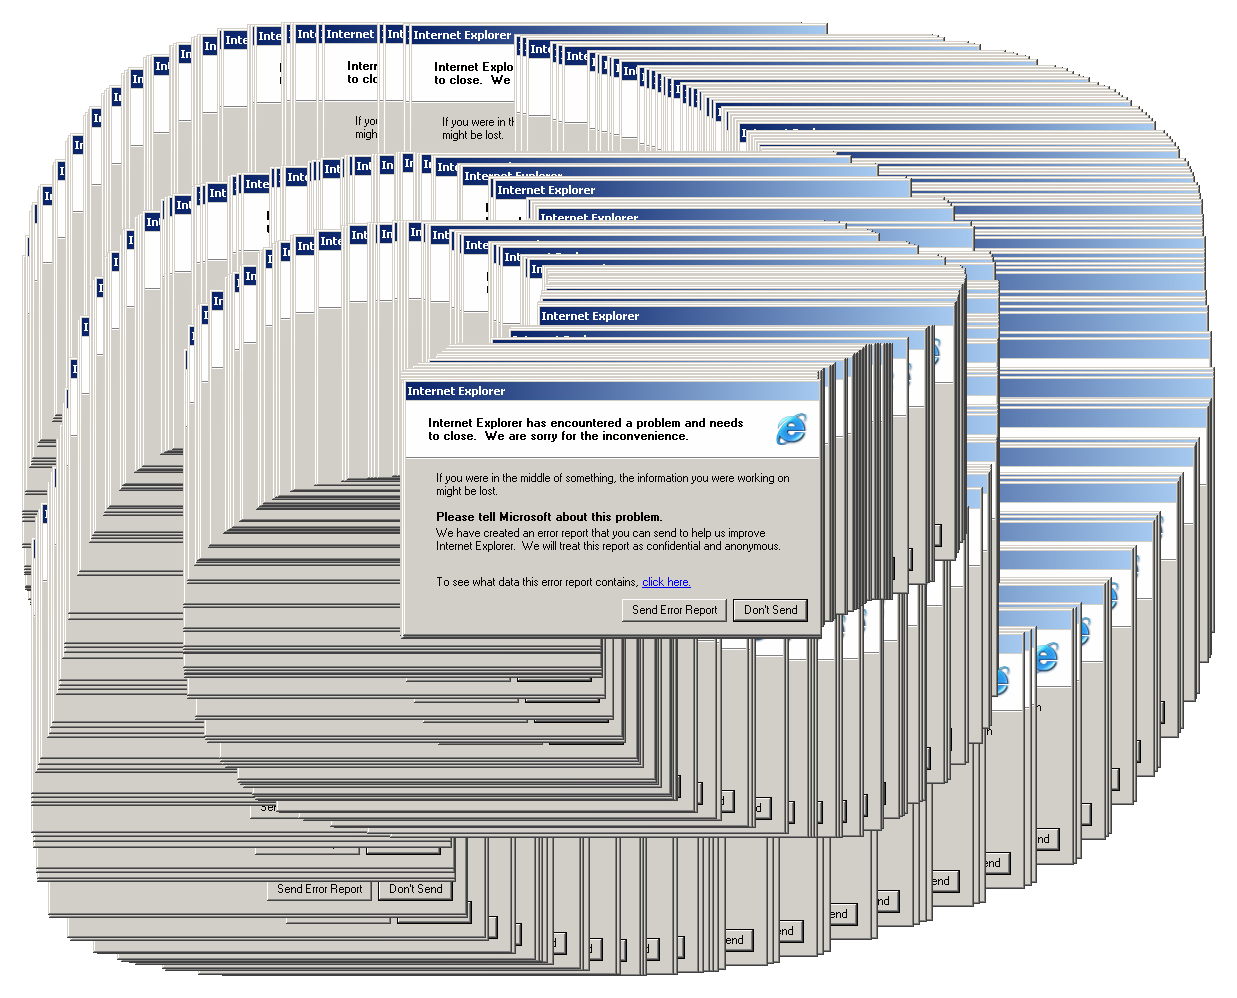
\includegraphics[width=0.8\columnwidth]{trail}
				\caption{The classic \enquote{trail} effect} % TODO: Reword
				\label{fig:trail}
			\end{figure}

			Another shortcoming of non-compositing window managers is their
			inability to provide visual effects. As a consequence of the fact
			that (at most) one application determines the color of each individual
			pixel on the screen, effects such as partially transparent windows
			cannot be realized with non-compositing window managers. Additionally,
			because a window may only be at most at one position of the screen,
			and that position has to be the Window's \enquote{actual} position,
			no thumbnails or overviews of windows can be shown.

			Compositing is an attempt at a solution to the aforementioned
			problems.  If a compositing window manager is in use, applications
			do not draw directly to the screen. Instead, each applications has
			its own off-screen buffer. The
			window manager then assembles the final
			desktop from the content of these buffers. It is immediately clear how this approach addresses the
			problems of non-compositing window-managers described above: It is
			easy to perform double buffering and even when a window is not
			responding, the window manager knows its last good state and can
			use it to prevent trails. Furthermore, visual effects are trivial
			to achieve when compositing is used. \cite{dwmoverview}

		\subsection{The Desktop Window Manager\winver{V}}\label{sec:dwm}
			The \emph{Desktop Window Manager} (DWM) is the compositing window
			manager used by Windows and introduced in Longhorn
			\cite{dwmoverview}.  It is implemented as a full-screen Direct3D
			user-space application. In particular, DWM rendering is
			hardware-accelerated. When DWM is active, applications render into
			off-screen DirectX buffers which are mapped onto flat surfaces in
			3D space and rendered by the graphics hardware. This design enables
			three-dimensionally transforming the windows, which is used for the
			\enquote{Flip3D} feature of Windows Vista invoked by the keyboard
			shortcut \keys{Win+\tab} and its more modest counterparts in more
			recent versions of Microsoft Windows. Visual effects such as
			transparency are implemented using DirectX pixel shaders. In addition,
			double buffering using a buffer flipping mechanism is implemented.
			\cite{dwmdirectx}

			Even though DWM is a native application, its implementation closely
			resembles that of an Avalon application. In particular, the desktop
			is modeled as a visual tree in the same way that WPF applications
			are modeled as a visual tree (refer to section~\ref{sec:milcore}
			for details) and also uses \texttt{milcore.dll} to render the
			visual tree through DirectX. This code reuse provides a
			substantial number of necessary functional and performance
			features essentially for free.  In particular, the visual tree
			model, which at first might appear not to fit a mostly
			non-hierarchical situation such as the desktop, very well,
			turns out to be very beneficial, since the Avalon composition
			engine comes with support for \emph{occlusion culling}---i.e.,
			determining which parts of a window are visible at a particular
			moment. This feature completely takes care of the task to
			determine which parts of a window should be drawn. Similarly, the
			entire logic that decides when to request which region of which window
			to redraw (scheduling and dirty region management) is taken from
			Avalon.
			\cite{dwmwpf}

			The way in which windows are redirected when DWM is in use depends
			on the drawing API used by the application. GUI applications which
			(directly or indirectly)
			use DirectX for rendering can render into a single buffer located
			in video memory allocated
			by the DWM. Because DWM itself uses DirectX, DirectX applications
			natively render into the format used by DWM, so the DWM can use
			these buffers directly to perform composition. Sharing a single buffer
			between an application and DWM is not natively supported by DirectX
			but a WDDM feature; refer to section~\ref{sec:wddm} for details.
			\cite{dwmredirect}

			Applications employing GDI for their rendering cannot render into
			the DirectX pixel format, but render into a DWM-provided main memory
			buffer in their native GDI format. When the window is created, DWM
			automatically also creates a DirectX buffer in video memory. The
			application draws into the GDI buffer, and DWM manually transcribes
			the GDI buffer to the DirectX buffer when necessary and uses the result
			for composition.
			\cite{dwmredirect}

		\subsection{The Windows Display Driver Mo\-del\winver{V}}\label{sec:wddm}
			The implementation of DWM described in section~\ref{sec:dwm}
			fundamentally relies on graphics driver support in order to achieve
			reasonable performance.  Prior to Longhorn, DirectX applications
			assumed that they have exclusive access to the GPU. In particular,
			there was no virtual memory and no support for preemption. This is
			unproblematic as long as there is at most one active DirectX application
			and that application has reasonably predictable video memory requirements.
			However, the Desktop Window Manager \emph{is} a DirectX appliction that
			by design both runs alongside other DirectX applications and whose
			memory consumption is dependent on the number of open windows and therefore
			very unpredictable.
			In order to address these problems, display drivers targeting Longhorn
			have to be written against the Windows Display Driver Model. This
			display driver framework introduces the cooperative multitasking
			features known from regular applications running on the CPU to the
			GPU. \cite{dwmwddm}

			One of these features is an implementation of preemtion called
			WDDM \emph{scheduling}. The granularity of preemtion depends on
			the version of DirectX that is used and hardware support. When
			using \emph{Basic Scheduling}, available from DirectX 9 without
			special hardware support, primitives and shaders cannot be interrupted,
			so preemption can only take place inbetween these basic operations.
			If the hardware supports it and DirectX 10 is in use, \emph{Advanced
			Scheduling} is available, allowing preemption to take place in the mid
			of primities or shaders. \cite{dwmwddm}

			The other large feature required for cooperative multitasking is
			virtual memory. As GPUs may have several regions of video memory
			specialized for certain tasks, the address space of a GPU may
			be nonlinear. For this reason, the GPU announces some number of
			available segments of video memory to the driver framework \cite{gpuseg}.
			When using the WDDM 1.$x$ model for virtual graphics
			memory, applications work with segment physical addresses. In the event
			that a piece of memory is moved or paged out, addresses in the command
			buffer are patched. This model was updated to using proper virtual
			addresses with WDDM 2.0, introduced in Windows 10. \cite{wddm2}

			Finally, a third feature that is necessary to implement the redirection
			mechanism for DirectX applications described in section~\ref{sec:dwm}
			is DirectX surface sharing, which gives an application and the DWM
			access to the same DirectX surface buffer, so that the DWM can use the
			same surface for compositing that is used by the application for
			drawing to. \cite{dwmredirect}

			The desktop window manager cannot run without a WDDM-compliant
			display driver \cite{dwmwddm}. If no such driver is available, one
			of two things will happen, depending on the version of Windows that
			is running. Under Windows Vista and Windows 7, DWM will be
			disabled\footnote{In Windows Vista/7, there are some other ways for
			DWM to be disabled. Applications can disable the DWM manually (for
			example immediately before switching to full-screen mode)
			\cite{disabledwm}, or DWM can be automatically disabled by an
			application using the drawing APIs incorrectly \cite{dwmredirect}.}
			and the non-compositing window manager\footnote{Contrary to the DWM,
			the non-compositing window manager referred to as \textit{USER} resides
			in \texttt{win32k} and thus in kernel space \cite{probertwin32k}.}
			from Windows XP will be used. When running Windows 8 or later,
			the DWM will be run, but a software-based renderer called
			\textit{Microsoft Basic Display Adapter} will serve as a replacement
			for the display driver \cite{dwmalwayson}.


		\subsection{Hardware-accelerated GDI ren\-der\-ing\winver{7}}
			During Longhorn development, having GDI directly render to DirectX
			surfaces in video memory was deemed infeasible; not because GDI calls
			could not be adapted to work with the DirectX buffer format, but because
			GDI renders using the CPU and many GDI operations not only write to
			the buffer, but also need to read from it, but reading from video memory
			using the CPU is a very slow operation \cite{dwmredirect}. However,
			Windows 7 does eliminate the main memory buffer for GDI. The performance
			issues were resolved by providing explicit hardware acceleration for
			the offending GDI operations in WDDM version 1.1. In particular,
			starting with Windows 7, the
			main memory comsumption of the Desktop Window Manager is independent
			of the number of open windows (however, VRAM comsumption still scales
			linearly with the number of open windows).
			\cite{win7}

	\onecolumn{\printbibliography}
\end{document}
